\documentclass{article}

\usepackage{a4wide}
\usepackage[utf8]{inputenc}
\usepackage[T1]{fontenc}
\usepackage[french]{babel}
\usepackage[babel=true]{csquotes} % guillemets français
\frenchbsetup{ItemLabels=\textbullet}
\usepackage{graphicx}
\graphicspath{{Images/}}
\usepackage{color}
\usepackage{hyperref}
\hypersetup{colorlinks,linkcolor=,urlcolor=blue}

\usepackage{amsmath}
\usepackage{amssymb}
\usepackage{wrapfig}


\title{Rapport de projet Android}
\author{Arthur Wenger \and Shad Maleck}
\date{\today}

\begin{document}

\maketitle


\begin{abstract}
  Ce document est un rapport détaillant le développement d'un projet Android dans le cadre de la 1\iere\ année de master informatique à l'Université de la Réunion.
\end{abstract}

%\clearpage
%\tableofcontents

% Introduction --------------------------------
\section{Introduction}
Le projet présenté dans ce rapport concerne la création d'un jeu Android implémentant les fonctionnalités suivantes:\\
\begin{itemize}
  \item Le jeu utilise un accéléromètre pour déplacer un personnage à l'écran.
  \item Un score permet de déterminer la performance du joueur pendant une partie. 
  \item Un menu accessible en jeu permet d’afficher la liste des scores obtenus .
  \item Un clic sur un score de la liste affiche une carte centrée sur la position
  géographique où le score a été obtenu.
  \item Un marqueur est placé sur la position de chaque score et affiche la valeur du score obtenu ainsi que le couple (latitude, longitude) de la position.
  \item Les scores sont sauvegardés dans une base de données SQLite et sont donc persistants.
  \item Le jeu utilise un ensemble de fichiers de son qui sont joués lors évènements appropriés pendant une partie.
\end{itemize}~\\
Dans un premier temps nous nous pencherons sur la structure de l'application puis nous étudierons le détail du fonctionnement de chacune de ses fonctionnalités.

% Présentation de l'application --------------------------------
\section{Présentation de l'application}
% Principe du jeu --------------------------------
\subsection{Principe du jeu}
Le jeu implémenté dans cette application est une version modifiée du \textit{célèbre jeu Pacman}~\cite{pacmanDoc}.
Le principe du jeu original est simple: l'utilisateur contrôle le héro pacman et doit récupérer des pièces disséminées à l'intérieur d'un labyrinthe hantés par des fantômes.
L'objectif est de récupérer le maximum de pièces sans se faire toucher par les fantômes.\\

Notre version du jeu diffère cependant en quelques points.
\\Tout d'abord, les mouvements et la direction de pacman dépendent exclusivement de l'inclinaison du téléphone.
\\Par ailleurs, pacman dispose de deux vies quand il commence une partie et peut augmenter ce nombre en collectant des cœurs cachés dans le labyrinthe.
Chaque collision avec un fantôme retire une vie à pacman et le rend invulnérable pendant 3 secondes.
\\De plus, le nombre de fantômes dans le labyrinthe n'est pas limité à 4 comme le jeu standard. 
Ce nombre varie en fonction de la difficulté du jeu.
\\Une ligne d'arrivée est également placée aléatoirement dans le labyrinthe. 
Si pacman atteint cette ligne d'arrivée, le score du joueur augmente 20 points, la vitesse des fantômes est augmentée et un nouveau labyrinthe est généré.
\\Enfin, Les fantômes ne peuvent pas être mangés contrairement à la version originale du jeu.

% Structure des fichiers --------------------------------
\subsection{Structure des fichiers}
% les packages --------------------------------
\subsubsection{Les packages}
Le projet est divisé en packages correspondant à chacune des fonctionnalités de l'application:
%\begin{wrapfigure}{r}{5cm}
%  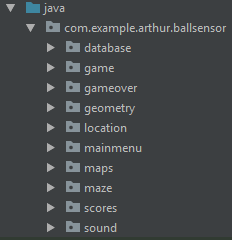
\includegraphics[width=5cm]{packages.png}
%\end{wrapfigure} 
\begin{center}
  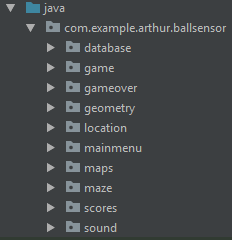
\includegraphics[width=5.5cm]{packages.png}
\end{center}
\begin{itemize}
  \item Le package \enquote{database} contient la classe \enquote{DBManager} permettant de manipuler la base de données SQLite de l'application.
  \item Le package \enquote{game} contient l'activité et la vue du jeu ainsi que les classes permettant de modéliser les objets du jeu.
  \item Le package \enquote{gameover} contient l'activité s'affichant à l'écran lorsque la partie est perdue.
  \item Le package \enquote{geometry} contient des classes permettant de manipuler et d'effectuer des opérations sur des formes géométriques simples dans un espace à deux dimensions.
  \item Le package \enquote{location} contient la classe \enquote{SingleShotLocationProvider} ainsi qu'un écouteur permettant de récupérer les coordonnées géographiques du téléphone.
  \item Le package \enquote{mainmenu} contient l'activité \enquote{MainActivity} permettant d'afficher la page d'accueil de l'application.
  \item Le package \enquote{maps} contient la classe \enquote{MapsActivity} nécessaire à l'affichage d'une carte Google Map montrant l'emplacement ou chaque score a été obtenu.
  \item Le package \enquote{maze} contient un ensemble de classes permettant d'afficher et de générer aléatoirement un labyrinthe pour le jeu.
  \item Le package \enquote{scores} contient les classes permettant de manipuler et d'afficher la liste des scores obtenus.
  \item Enfin, le package \enquote{sound} contient la classe \enquote{AudioPlayer} permettant de jouer des sons pendant le jeu.
\end{itemize}

% Les ressources --------------------------------
\subsubsection{Les ressources}
Les ressources du projet sont reparties dans deux dossiers:
\begin{center}
  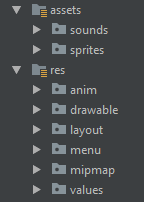
\includegraphics[width=3.5cm]{res.png}
\end{center}
\begin{itemize}
  \item Le dossier \enquote{assets} regroupe les ressources manipulées par le jeu. 
  Le sous dossier \enquote{sounds} contient l'ensemble des fichiers de son d'extension .ogg utilisés par le jeu.
  Le sous dossier \enquote{sprites} contient l'ensemble des images représentant les objets du jeu.
  \item Le dossier \enquote{res} contient les ressources standard manipulées par l'application: images pour l'écran d'accueil et les scores, fichiers xml de description des activités et des menus, chaines de caractères pour la traduction du texte en français et en anglais...\\
  Aux dossiers conventionnels pour Android s'ajoute également le dossier \enquote{anim} responsable de l'animation de transition de l'activité GameOver.
\end{itemize}

% L'écran d'accueil et les sons --------------------------------
\section{L'écran d'accueil et les sons}
% L'écran d'accueil --------------------------------
\subsection{L'écran d'accueil}
L'activité \enquote{MainActivity} du package \enquote{mainmenu} est le point d'entrée de l'application. 
Elle utilise le layout \enquote{activity\_main} pour afficher l'écran d'accueil:
\begin{center}
  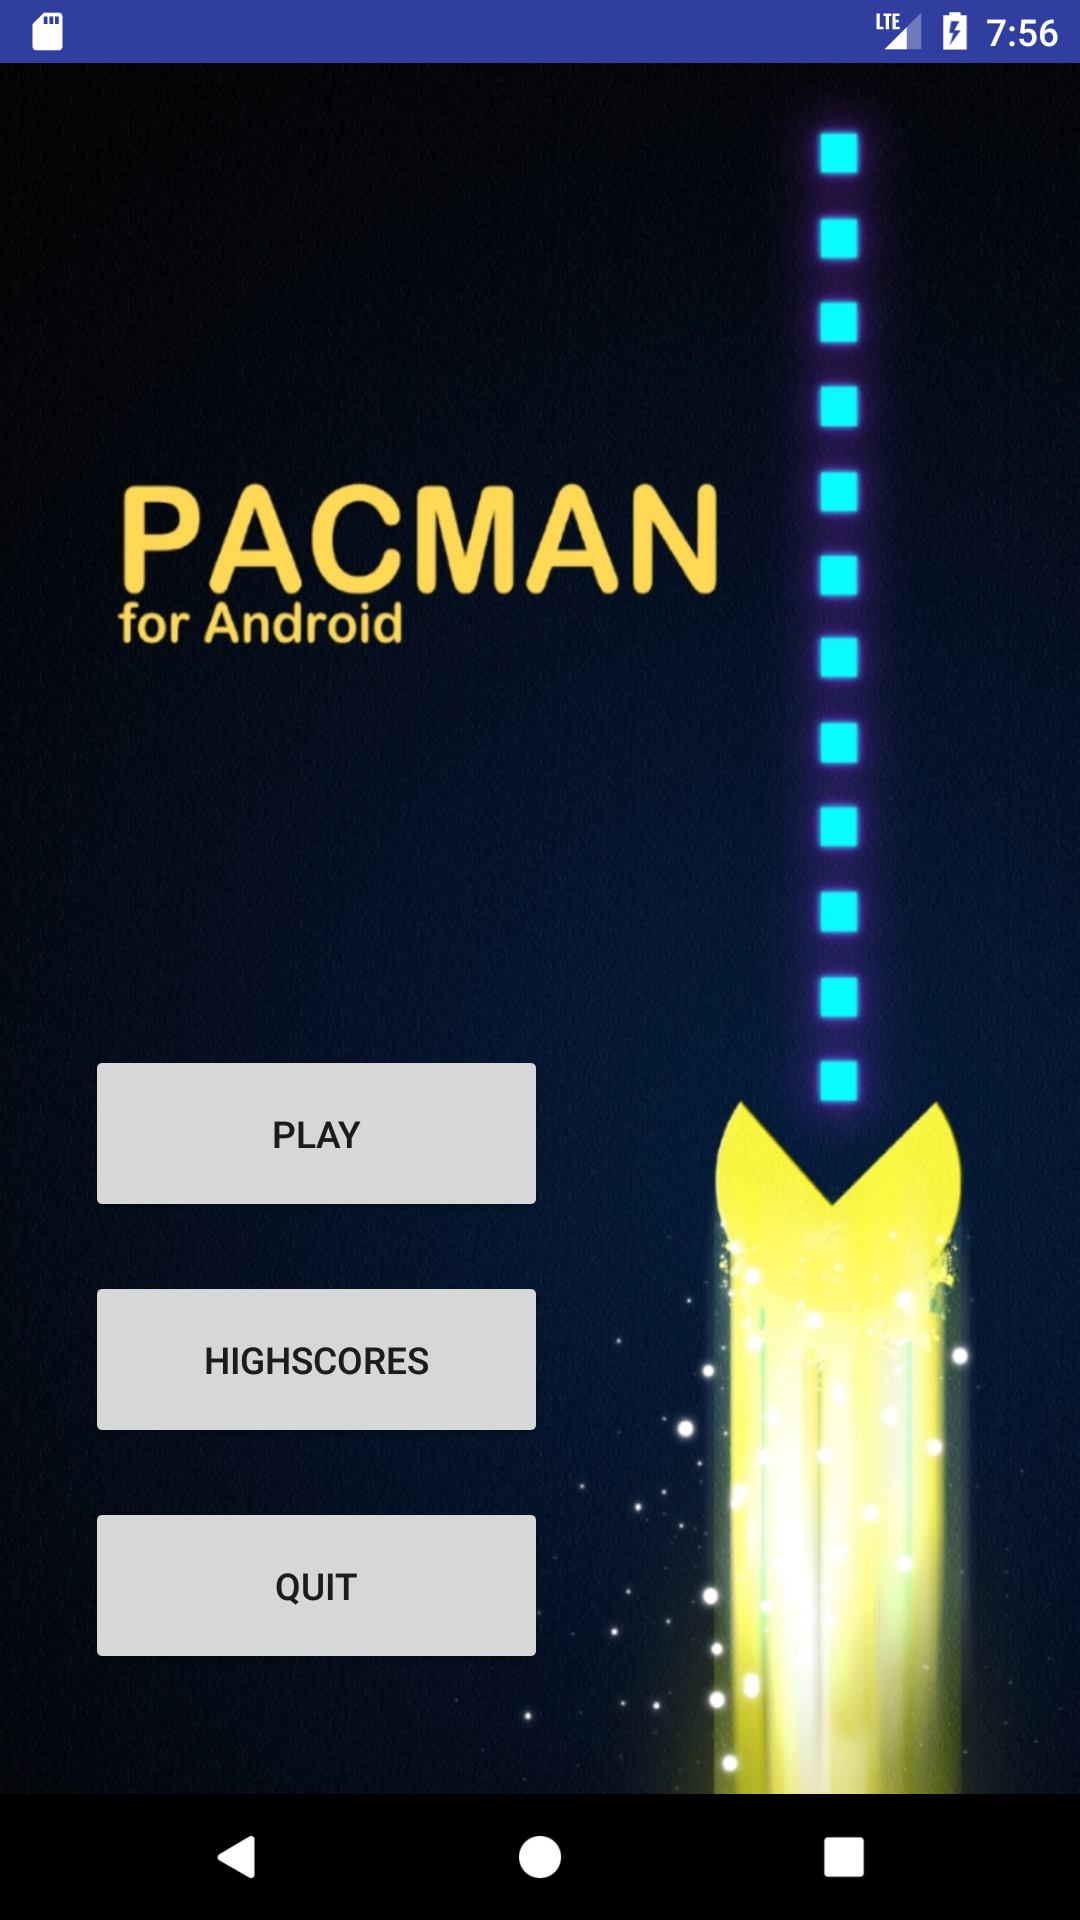
\includegraphics[width=5cm]{home_screen.png}
\end{center}
Au lancement de l'activité, une instance de la classe AudioPlayer est créée pour jouer le thème de Pacman:
\begin{verbatim}
  backgroundMusic = new AudioPlayer( this.getAssets() );
  backgroundMusic.startPlayer( "sounds/pacman_song.ogg", 1f, true);//On lance la musique de fond
\end{verbatim}
L'écran d'accueil propose trois options:
\begin{itemize}
  \item L'option Play lance une nouvelle activité \enquote{GameActivity} afin de commencer une nouvelle partie.
  \item L'option Highscores lance une nouvelle activité \enquote{ScoresActivity} afin d'afficher la liste des scores.
  \item L'option Quit permet de quitter l'application.
\end{itemize}

% Les sons --------------------------------
\subsection{Les sons}
L'ensemble des sons et des musiques du jeu sont stockés dans le dossier assets/sounds et sont manipulées par la classe \enquote{AudioPlayer} du package \enquote{sound}.
Cette classe encapsule une instance de MediaPlayer afin de jouer un son spécifique du dossier assets.
Les méthodes startPlayer et stopPlayer permettent respectivement de démarrer et arrêter le lecteur de son.
L'intérêt de cette classe par rapport à une utilisation directe de MediaPlayer réside dans la libération automatique des ressources allouées pour la lecture des sons.
En effet, lorsqu'un son se termine ou lors d'un appel à la méthode startPlayer, l'instance de la classe MediaPlayer manipulée par la classe AudioPlayer libère systématiquement ses ressources. 


% L'affichage du jeu --------------------------------
\section{L'affichage du jeu}

Le package \enquote{game} contient les classes modélisant les objets du jeu ainsi qu'une activité utilisant une vue personnalisée pour l'affichage du jeu:
\begin{center}
  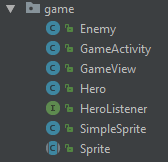
\includegraphics[width=4cm]{game_package.png}
\end{center}

% L'activité GameActivity --------------------------------
\subsection{L'activité \enquote{GameActivity}}
L'activité \enquote{GameActivity} gère l'affichage de la fenêtre du jeu. L'affichage du jeu est délégué à la vue \enquote{GameView} qui est au centre de l'activité.\\
Les fonctions de l'activité \enquote{GameActivity} sont multiples.\\

Tout d'abord, elle initialise le menu du jeu à l'aide de la fonction onCreateOptionsMenu qui utilise un layout comprenant trois options: l'affichage des scores, le lancement d'une nouvelle partie et le retour à l'écran d'accueil:
  \begin{verbatim}
  public boolean onCreateOptionsMenu( Menu menu ) {
    getMenuInflater().inflate( R.menu.game, menu );
    return true;
  }
  \end{verbatim}

Ensuite elle met en place un écouteur sur un accéléromètre dont elle transmet les mise à jour à la vue \enquote{GameView}:
  \begin{verbatim}
  private class MySensorListener implements SensorEventListener {
    @Override
    public void onSensorChanged( SensorEvent event ) {
      if (event.sensor.getType() != Sensor.TYPE_ACCELEROMETER)
        return;
      else
        mazeView.updateAccel( -event.values[0], event.values[1]);
    }
  }
  \end{verbatim}

Lors de son initialisation, elle fait également appel à la classe \enquote{SingleShotLocationProvider} afin de récupérer la position du téléphone au lancement d'une partie.
Cette position sera utilisée par l'activité GameOver afin d'enregistrer le score obtenu par l'utilisateur dans la base de données.
Celle-ci est récupérée au lancement du jeu et non lors d'un Game Over en raison des délais et des eventuelles demandes de permission qui peuvent retarder l'acquisition de la position du téléphone.\\

Par ailleurs, cette activité met en place deux écouteurs. 
L'écouteur \enquote{GameOverListener} lui permet de lancer l'activité \enquote{GameOver} lorsque la vue centrale lui informe que la partie est perdue.
L'écouteur \enquote{LocationListener} lui permet de réagir aux évènements de la classe \enquote{SingleShotLocationListener}.\\

Enfin, cette activité gère les évènements sur le menu d'options du jeu ainsi que les codes de retour des activités \enquote{GameOver} et \enquote{ScoresActivity} susceptibles d'être lancées par cette activité.
La méthode onOptionsItemSelected définie le comportement de l'application lors des clics sur les options du menu tandis que la méthode onActivityResult permet de reprendre le jeu, lancer une nouvelle partie ou quitter l'activité en fonction des codes de retour des activités appelées.


% La vue GameView --------------------------------
\subsection{La vue \enquote{GameView}}
La vue \enquote{GameView} redéfinie la méthode d'affichage onDraw afin de dessiner le labyrinthe et les objets du jeu à l'écran:
\begin{center}
  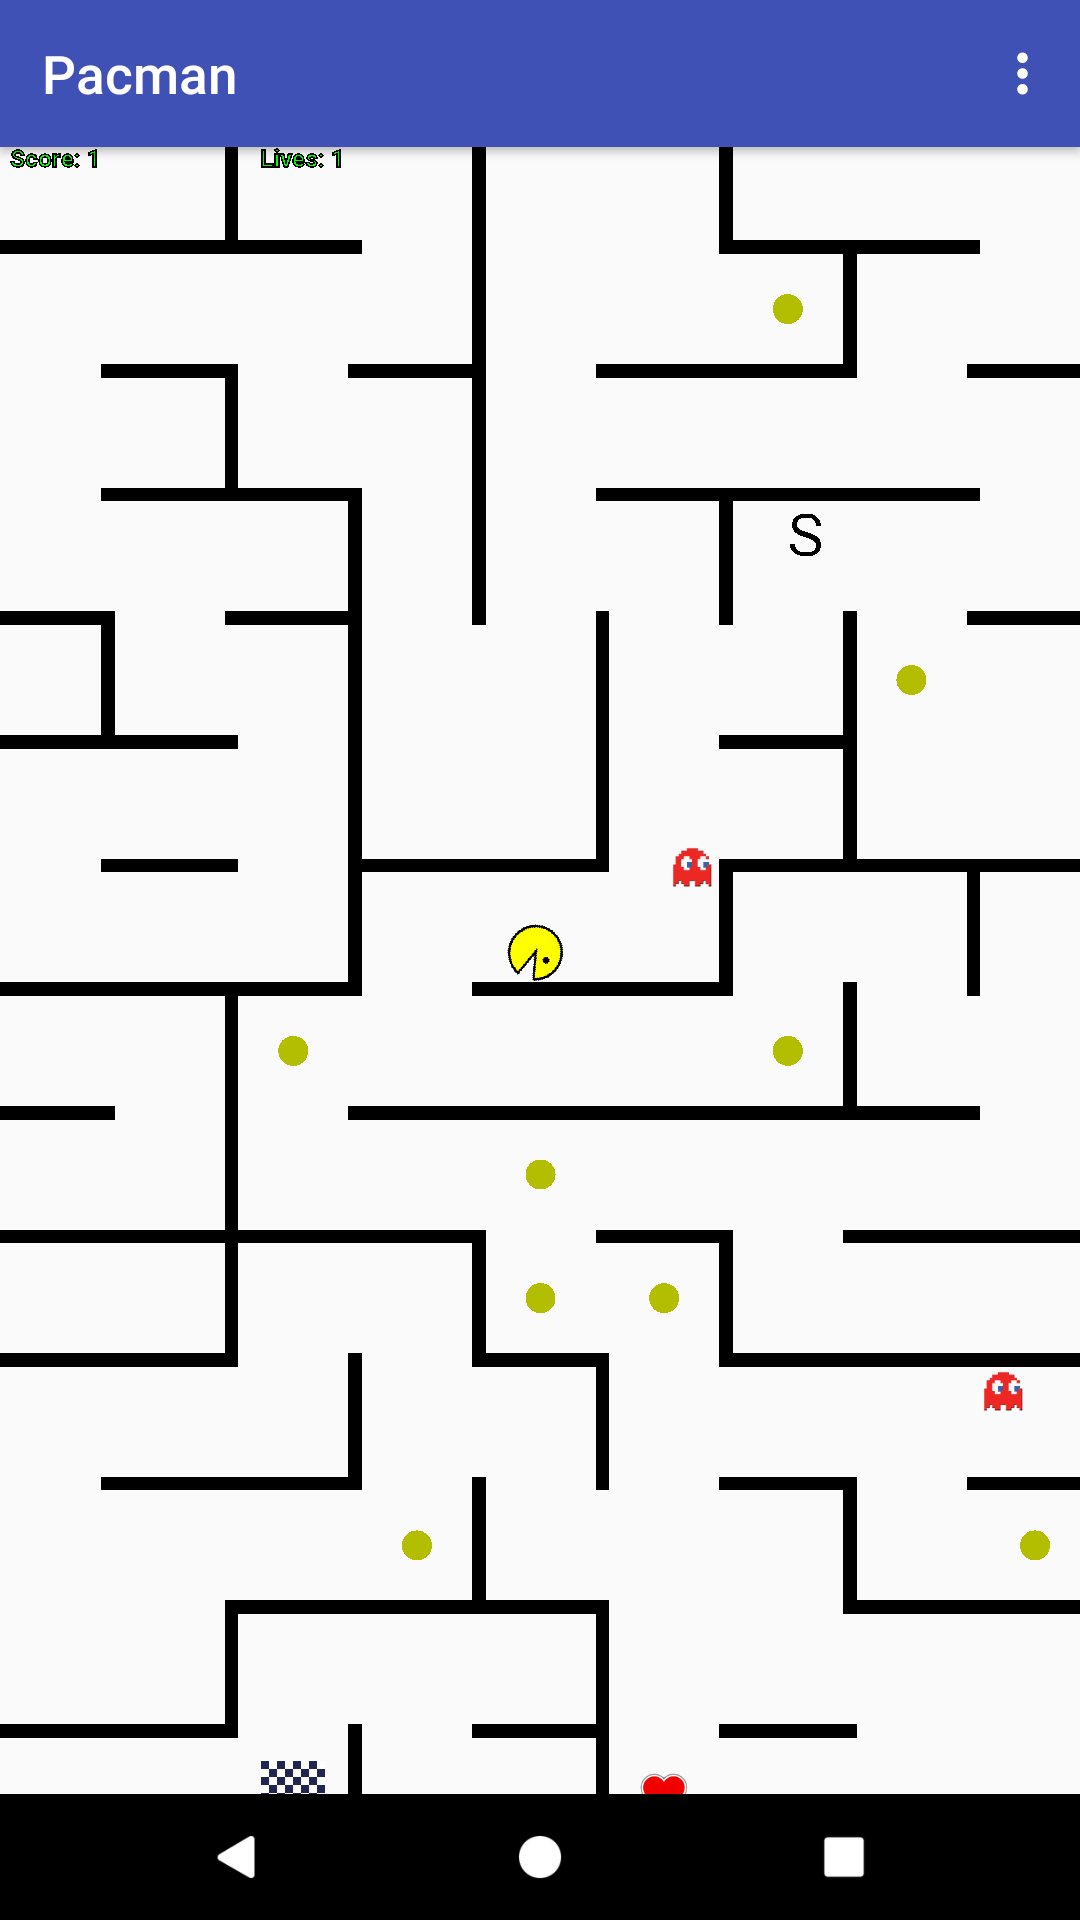
\includegraphics[width=5cm]{game_screen.png}
\end{center}
L'initialisation des éléments composant le jeu est effectuée avec la méthode generateMaze. 
Celle-ci utilise une instance de la classe \enquote{DepthFirstSearchMazeGenerator} afin de générer aléatoirement un labyrinthe de dimensions spécifiques à l'écran.
Ce labyrinthe nous permet d'initialiser les positions des ennemis, du joueur, de la ligne d'arrivée ainsi que des objets récupérables en jeu.\\

La classe interne \enquote{UpdateTimerTask} hérite de la classe TimerTask et permet de mettre à jour les objets du jeu à intervalle régulier.
Cet intervalle est défini par les les constantes FPS et FramePeriod qui imposent au jeu un taux de rafraichissement de 30 images par secondes.
A chaque mise à jour du jeu, les méthodes update des objets mobiles sont appelées afin de les déplacer dans le labyrinthe.
Les collisions entre le héro, les ennemis, les murs et les objets récupérables sont détectées à l'aide des méthodes detectAndResolveCollision des classes \enquote{Hero} et \enquote{Ennemy}.
Enfin, un effet de caméra est simulé afin de focaliser l'attention du joueur sur la partie du labyrinthe dans lequel se trouve pacman.
Cette caméra dispose d'un mouvement propre qui est mis à jour en même temps que les objets du jeu.\\

La méthode onDraw fait appel aux méthodes draw de chacun des objets du jeu afin de la afficher à l'écran.
Les objets récupérables dans le labyrinthe doivent être synchronisés afin d'éviter des problèmes d'accès concurrent par la classe UpdateTimerTask.\\

La méthode updateAccel permet de mettre à jour les valeurs accélérations ponctuelles de pacman en fonction des données fournies par l'accéléromètre.

Les méthodes stopTimer et startTimer permettent respectivement de mettre le jeu en pause et de reprendre le jeu.
La méthode newGame permet quant à elle de lancer une nouvelle partie en générant un nouveau labyrinthe et en réinitialisant les objets du jeu.\\

Enfin, cette vue implémente l'interface \enquote{HeroListener} pour écouter les événements se produisant sur pacman.
En particulier, lorsque pacman notifie la vue qu'il vient de mourir avec la méthode notifyHeroDeath, celle-ci en informe l'activité \enquote{GameActivity} afin qu'elle affiche un écran de Game Over.

% L'écran de game over --------------------------------
\subsection{L'écran de game over}
L'écran de game over est affiché grâce l'activité \enquote{GameOverActivity} du package \enquote{gameover}:
\begin{center}
  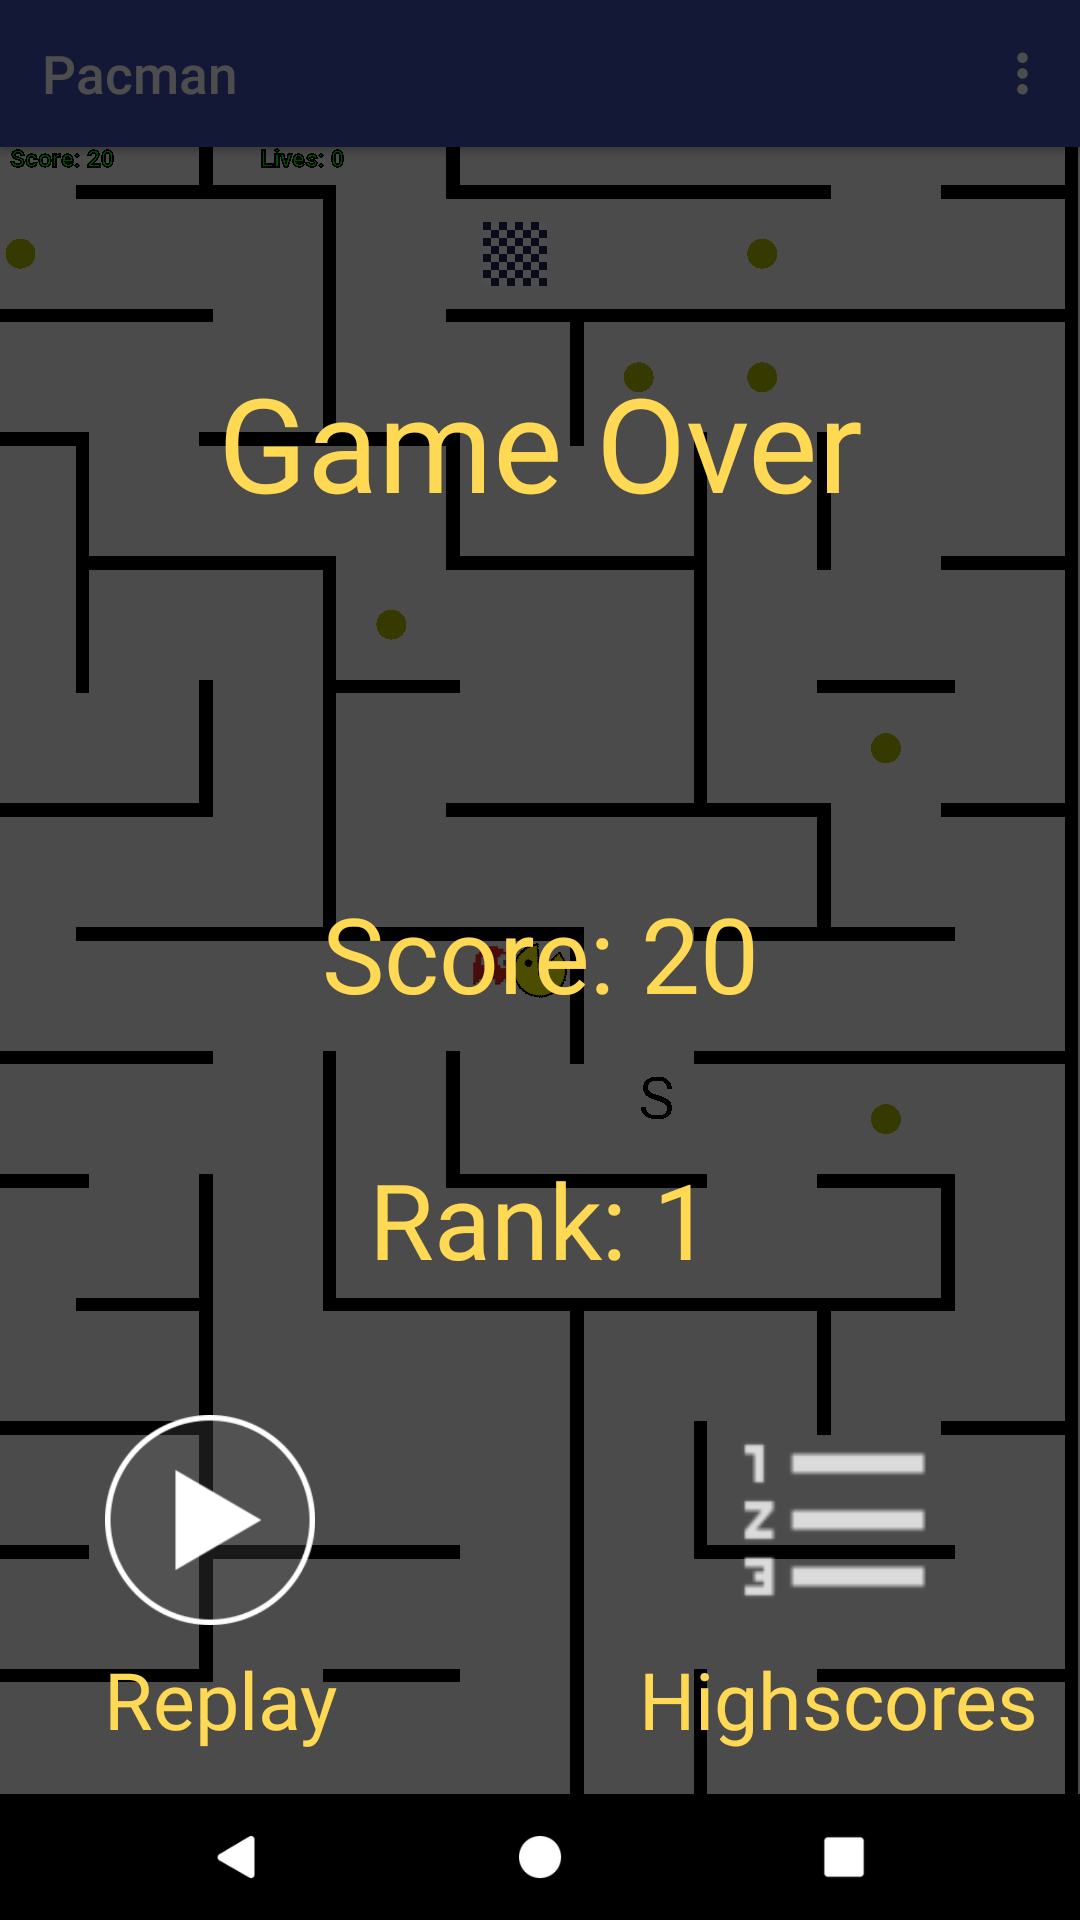
\includegraphics[width=4cm]{game_over.png}
\end{center}
Cette activité utilise une couleur de fond semi transparente afin de donner l'illusion qu'elle se superpose au jeu.
Deux options permettent respectivement de rejouer une partie et d'afficher la liste des scores obtenus.\\

Le score du joueur est transmis par l'activité \enquote{GameActivity} à la fin de la partie.
Le rang du joueur est récupéré avec la méthode getRank de la classe \enquote{DBManager}.
Une requête SQL simple récupère l'ensemble des scores supérieurs ou égaux au score obtenu par le joueur puis calcule son rang.\\

% Les objets du jeu --------------------------------
\section{Les objets du jeu}
% Les sprites --------------------------------
\subsection{Les sprites}
La classe abstraite \enquote{Sprite} définie un ensemble d'attributs et de méthodes permettant de manipuler les images représentant les objets du jeu.
En effet, la quasi totalité des objets du jeu sont représentés par une ou plusieurs images contenues dans le dossier \enquote{assets/sprites}.\\

Pour simplifier les calculs de collisions, chaque objets du jeu est virtuellement associé à une forme géométrique.
Par exemple, pacman et les fantômes sont associés à des cercles dont le diamètre est identique à la largeur de leurs sprites.
Ainsi, pour savoir si pacman vient d'entrer en collision avec un des fantômes, il suffit de vérifier que la distance qui sépare leurs centres est inférieure à la somme des rayons des cercles auquels ils sont associés.\\

La vitesse et la position des sprites sont définies par les attributs center, velocity et radius. 
Par ailleurs, une méthode detectAndResolveWallCollision permet de détecter une collision avec un mur en utilisant la méthode circleIntersectionResolutionOffset de la classe \enquote{LineSegment2D}.

La classe \enquote{SimpleSprite} sert à modéliser les objets immobiles du jeu représenté par une seule image.
Cette classe est essentiellement utilisée pour dessiner les objets récupérables en jeu mais aussi pour la ligne d'arrivée du labyrinthe.\\

% La classe Hero --------------------------------
\subsection{La classe Hero}
Les objets mobiles du jeu c'est-à-dire pacman et les fantomes disposent de leur propre classe.
Celles-ci héritent de la classe \enquote{Sprite} afin d'implémenter des méthodes de déplacement et d'affichage spécifiques.\\

La classe \enquote{Hero} modélise pacman. 
Celui-ci est représenté par une série de 7 sprites afin créer un effet d'animation à l'écran:
\begin{center}
  
\includegraphics[width=4cm]{pacman_sprites.png}
\end{center}
Chacune des images représentant pacman apparaît à intervalle régulier à l'aide d'une simple fonction modulo.
L'image appropriée est ensuite récupérée de l'ensemble des sprites à l'aide du numéro de l'animation en cours:
\begin{verbatim}
  animationFrameIndex = ( drawCounter / moveAnimationDrawsPerFrame ) % moveAnimationNumFrames;
  int srcLeft = pacmanSpriteWidth * animationFrameIndex;
  // les variables pacmanSpriteWidth et pacmanSpriteheight représentent 
  // la largeur et la hauteur d'une image
  Rect src = new Rect( srcLeft, 0, srcLeft + pacmanSpriteWidth, pacmanSpriteHeight );
\end{verbatim}
Le déplacement de pacman dépend exclusivement de la valeur d'accélération fournie par l'accéléromètre du téléphone.
L'accélération représentant une variation de vitesse, la valeur de la vitesse de pacman est calculée en fonction de la valeur de son accélération ponctuelle selon la formule:
$ v_f = v_i + a*dt $
L'intervalle de temps séparant deux affichages successifs étant constant (1/FPS), on peut simplement augmenter la vitesse de pacman d'une fraction de la valeur de son accélération.\\

Afin d'améliorer la fluidité et le réalisme des mouvements de pacman, une force de frottement est simulée et prise en compte dans la valeur de vitesse selon la formule: $v = v * ( 1 - drag * dt)$ 
La position du centre de pacman est ensuite modifiée en fonction de la valeur de sa vitesse actuelle.\\

De la même manière, des valeurs de vitesse et d'accélération angulaire permettent de faire tourner progressivement le sprite de pacman dans la direction vers laquelle il avance.

Enfin, quatre méthodes spécifiques permettent de jouer un son lorsque pacman entre en collision avec un fantôme, une pièce, un cœur ou lorsqu'il meurt.

% La classe Enemy --------------------------------
\subsection{La classe Enemy}
La classe \enquote{Enemy} modélise un fantôme dans le jeu.
A la différence de la classe \enquote{Hero}, cette classe ne dispose que d'un sprite représentant un fantôme.
Il serait cependant aisé d'ajouter une animation pendant le déplacement des fantômes en procédant de la même manière que pour pacman.\\

Le mouvement des fantômes est extrêmement simple.
Tous les fantômes ont la même vitesse au lancement du jeu.
Celle-ci est susceptible d'augmenter lorsque le joueur atteint la ligne d'arrivée du labyrinthe.
A chaque fois qu'un fantôme entre en collision avec un mur, il calcule la distance la plus courte permettant de rejoindre pacman et met à jour sa vitesse afin de se déplacer dans cette nouvelle direction:
\begin{verbatim}
  PointF distVector = Math2D.subtract( hero.getCenter(), getCenter() );
  float absX = Math.abs( distVector.x );
  float absY = Math.abs( distVector.y );
  if(absX >= absY){
    velocity.x = (distVector.x>0)? dirVelocity : -dirVelocity;
    velocity.y = 0;
  } else{
    velocity.x = 0;
    velocity.y = (distVector.y>0)? dirVelocity : -dirVelocity;
  }
\end{verbatim}
Chaque fantôme ne peut donc se déplacer qu'horizontalement ou verticalement à travers le labyrinthe.
Le problème majeur de cette méthode de déplacement vient du fait qu'elle ne prend pas en compte les chemins disponibles pour rejoindre pacman.
La conséquence directe est que les fantômes peuvent peuvent rester coincés sur une partie du labyrinthe en attendant que le joueur soit à proximité.
L'avantage de cette méthode réside néanmoins dans le fait que chaque fantôme peut être évité sans trop de problème au début du jeu.\\

Pour améliorer le déplacement des ennemis il faudrait créer une méthode de détection des intersections dans le labyrinthe ainsi qu'une méthode récupérant la liste des directions disponibles à un instant donné.
La direction du fantôme serait ainsi recalculée à chaque intersection pour lui permettre de minimiser la distance qui le sépare de pacman.
Ce type d'implémentation risque cependant d'élever considérablement la difficulté du jeu.

% Les scores et la carte --------------------------------
\section{Les scores et la carte}
% Les scores --------------------------------
\subsection{Les scores}
Les scores du jeu sont modélisés par la classe \enquote{Score} du package \enquote{scores}.
Cette classe contient quatre attributs représentant les caractéristiques d'un score:\\
\begin{itemize}
  \item L'attribut rank permet de mémoriser le classement du score obtenu par rapport à l'ensemble des scores de la base.
  \item L'attribut value permet de conserver la valeur du score obtenu.
  \item Enfin, les attributs lat et lng permettent de mémoriser la position géographique de l'appareil au moment ou le score a été obtenu.\\
\end{itemize}

L'activité \enquote{ScoresActivity} utilise une ListView afin d'afficher la liste des scores obtenus dans le jeu.
Tout d'abord, la liste des scores est récupérée puis stockée dans une ArrayList avec la méthode getAllScores de la classe \enquote{DBManager}. 
Une instance du contrôleur \enquote{ScoresArrayAdapter} est ensuite associé à la ListView afin de réaliser l'interface entre la vue et les données:
\begin{center}
  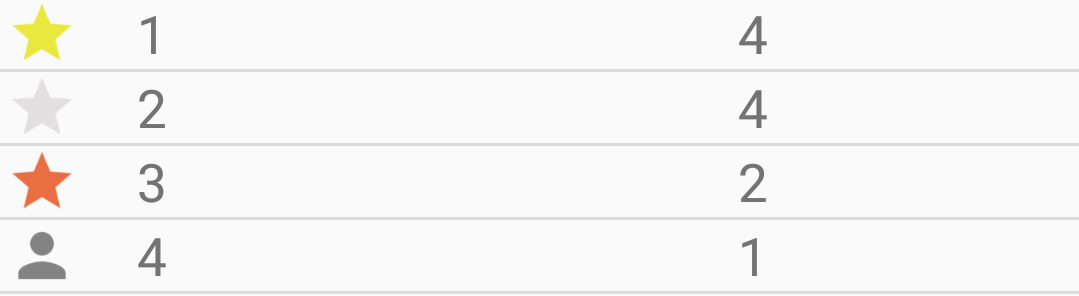
\includegraphics[width=4cm]{scores_list.png}
\end{center}

Le contrôleur \enquote{ScoresArrayAdapter} utilise le layout \enquote{cell\_layout} afin d'afficher les données de chaque score.
Chaque ligne de la liste comprend une icône, un rang ainsi qu'une valeur récupérée à partir des attributs de la classe \enquote{Score}. 
Les trois meilleurs scores disposent d'une couleur et d'une icône spécifique en forme d'étoile.
Si la liste des scores est affichée suite à un game over, la valeur du score obtenu par le joueur est surlignée en bleu.
La conversion du fichier XML \enquote{cell\_layout} décrivant chaque ligne de la liste et l'intégration des données de chacun des scores est réalisé par la méthode getView de la classe \enquote{ScoresArrayAdapter}. 

% La carte --------------------------------
\subsection{La carte}
L'affichage d'une carte Google Map est gérée par l'activité \enquote{MapsActivity} du package \enquote{maps}.
Cette carte est affichée uniquement lorsque l'utilisateur clique sur un des scores de la liste des scores.
L'activité appelante transmet alors à l'activité \enquote{MapsActivity} les coordonnées du score sur lequel l'utilisateur a cliqué tout en fournissant par la même occasion la liste des scores de la base.
Une carte utilisant l'API Google Maps est alors affichée à l'écran:
\begin{center}
  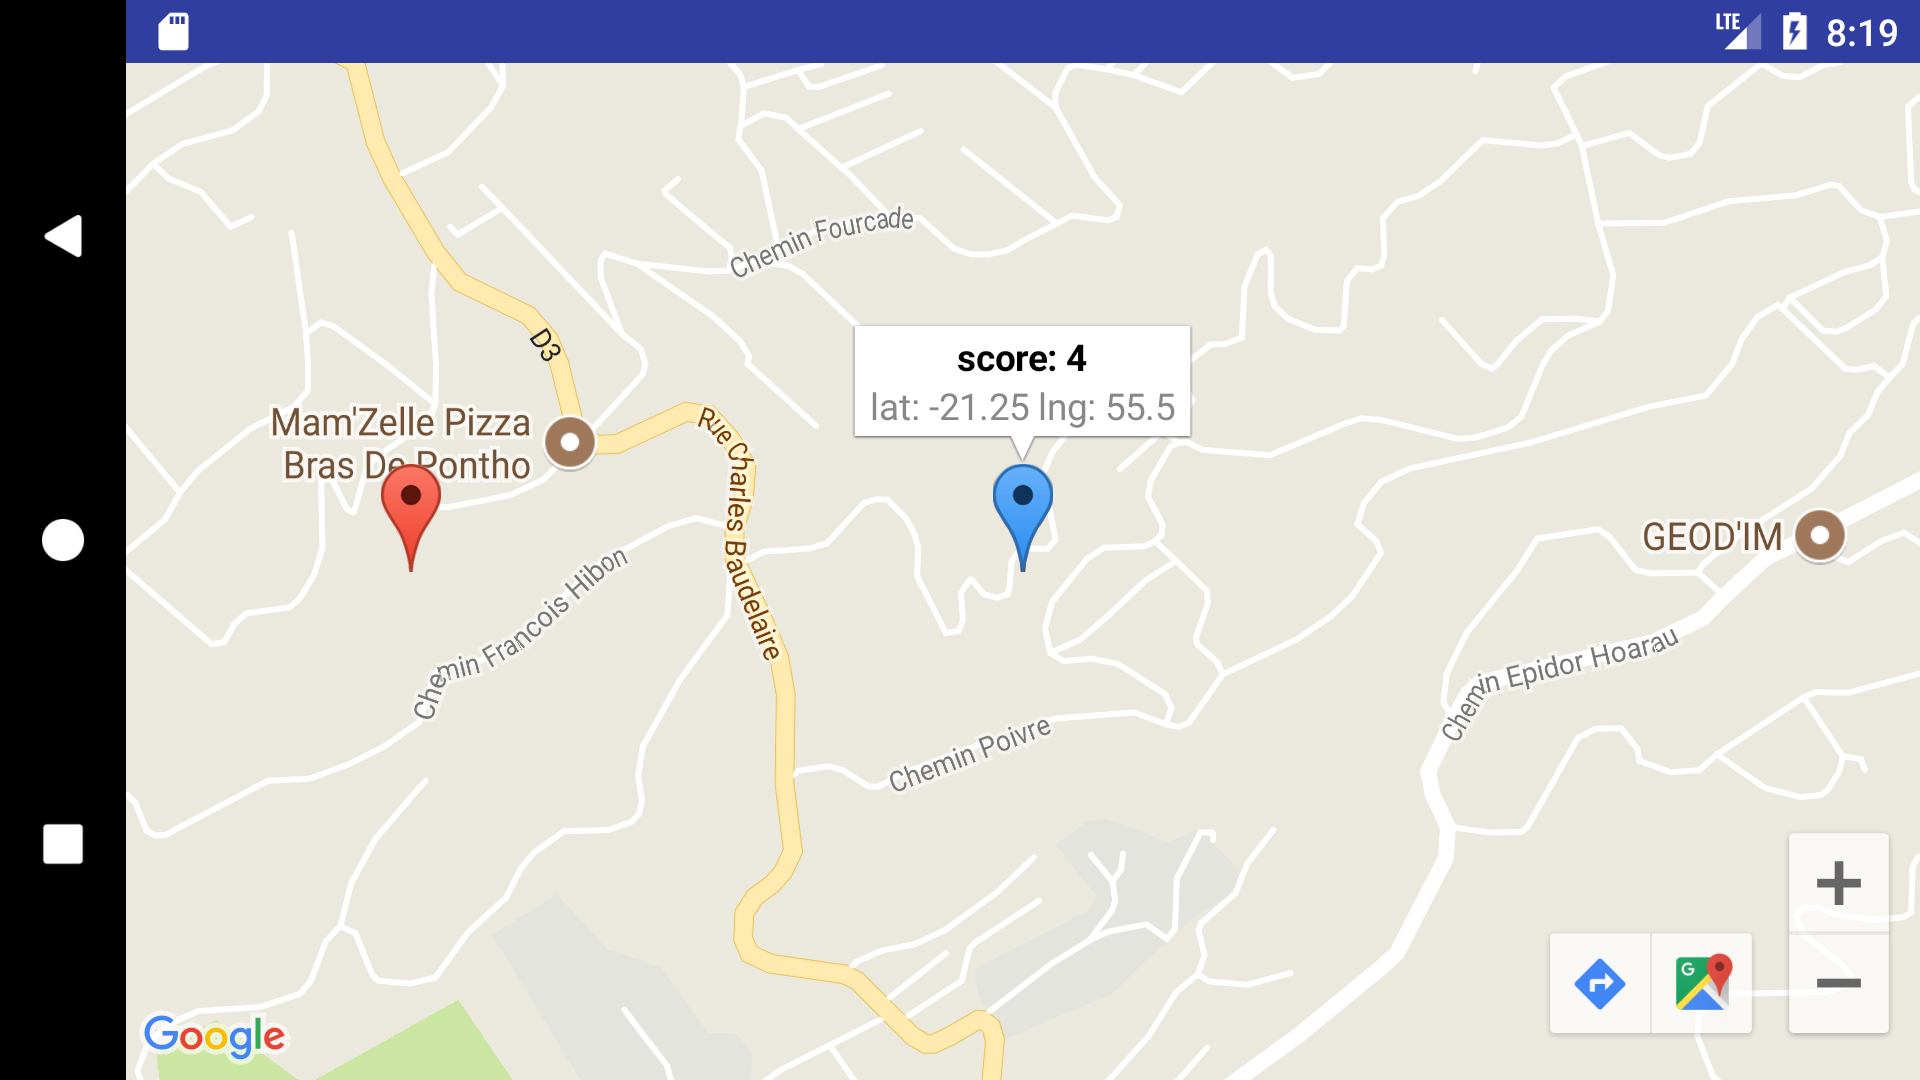
\includegraphics[height=4cm]{map_marker.png}
\end{center}

Les fonctionnalités implémentées par cette carte se limitent au stricte minimum.
Un ensemble de marqueurs indiquent la position de chaque score obtenu dans le jeu.
La carte est centrée sur un marqueur bleu qui représente le score sur lequel l'utilisateur a cliqué:
\begin{verbatim}
  mMap.animateCamera( CameraUpdateFactory.newLatLngZoom( centerLatLng, 11 ) );
\end{verbatim}

% Le labyrinthe et la modélisation 2D --------------------------------
\section{Le labyrinthe et la modélisation 2D}
% La géométrie du jeu --------------------------------
\subsection{Les calculs géométriques}
La classe \enquote{Math2D} du package \enquote{geometry} permet de comparer et d'effectuer des opérations sur des formes géométriques.\\

Elle implémente notamment un ensemble de méthodes de manipulations de vecteurs.
Un vecteur est modélisé par la classe PointF de la librairie graphics qui contient essentiellement les coordonnées de ce vecteur dans un espace à deux dimensions.
La classe \enquote{Math2D} définie ainsi des méthodes d'addition, de soustraction, de multiplication ou encore de produit scalaire sur les vecteurs.
Ces opérations basiques sont essentielles aux différents calculs de vitesse, d'accélération et de déplacement des objets du jeu.\\

Par ailleurs, cette classe définie des méthodes évaluant si deux formes géométriques s'intersectent.
En particulier, la méthode circleIntersection est extrêmement utile pour détecter les collisions entre les objets du jeu.
Cette méthode compare la distance séparant le centre de deux cercles à la somme de leurs rayons afin de déterminer s'ils sont en collision.\\

La classe \enquote{LineSegment2D} permet quant à elle de modéliser un mur dans le labyrinthe du jeu.
Ce mur est caractérisé par deux points formant une ligne.
La méthode intersectsCircle de cette classe est particulièrement utile pour déterminer les collisions des objets du jeu avec les murs du labyrinthe.
L'\textit{algorithme}~\cite{wallCollisionDoc} utilisé est décrit en détail dans les annexes.
Il consiste à comparer la distance du centre du cercle au pied de la perpendiculaire au segment.

% La génération du labyrinthe --------------------------------
\subsection{La génération du labyrinthe}
A chaque nouvelle partie, le jeu génère aléatoirement un labyrinthe avec la classe \enquote{DepthFirstSearchMazeGenerator} du package \enquote{maze}.
La génération de ce labyrinthe est basée sur l'algorithme \textit{Depth-First Search}~\cite{mazeDoc}.
Le principe est simple: l'espace alloué pour le jeu est divisé en cases de tailles égales, créant ainsi une grille.
Chaque case dispose initialement de quatre murs qui la sépare des cases adjacentes.
Pour créer le labyrinthe, on part d'une case choisie arbitrairement et on cherche à rejoindre une case voisine aléatoirement.
Pour rejoindre cette case on supprime le mur qui les sépare et on marque ces deux cases comme étant visitées.
On réitère ensuite ce procédé sur la case voisine jusqu'à ce qu'on atteigne une case dont toutes les cases voisines ont été visitées.
Dans ce cas, on revient en arrière et on continue l'algorithme sur une case qui a encore des voisins non visités.
L'algorithme s'arrête quand l'ensemble des cellules du labyrinthe ont été visitées.\\

Les murs du labyrinthe sont modélisés par la classe \enquote{LineSegment2D} du package \enquote{geometry}.
Ceux-ci sont placé sur les murs virtuels restant sur chacune des cases du labyrinthe à la fin de l'algorithme.\\

Enfin, la méthode getRandomRoomLocation de la classe \enquote{DepthFirstSearchMazeGenerator} permet de récupérer un ensemble d'emplacement libres dans le labyrinthe afin de pouvoir placer d'éventuels objets du jeu.

% Conclusion --------------------------------
\section{Conclusion}
Ce projet nous a permis de comprendre les différentes étapes liées à la création d'un jeu sur Android: de la création des images à l'implémentation des modèles en passant par la modélisation d'une surface de jeu.
Nous avons pu représenter et coordonner un ensemble d'objets utilisant des processus distincts dont l'interaction est régie par des calculs mathématiques s'apparentant à un moteur physique simpliste.
Nous avons également pu découvrir les principes fondamentaux des animations et des sprites utilisés pour afficher les objets d'un jeu.\\

Au travers de cette application, nous avons pu comprendre comment un ensemble d'activités peuvent communiquer et coopérer pour fournir différentes fonctionnalités telles que l'affichage d'une carte ou d'une liste de scores.
Il est intéressant de constater avec quelle facilité il est possible de tirer profit des nombreuses possibilités offertes par un téléphone comme les capteurs, le gps ou encore la connexion internet afin de construire une application.

%%% La bibliographie:
\bibliographystyle{plain}
\bibliography{ma_biblio}


\end{document}
